\graphicspath{{./images/chap7/}}
% Classification with CNN
% Methodology
% * Design and Architecture
% * Population of interest and sampling subject used in the study
% * Instrument and what it measures (metrices)
% * qualifications of informants if used in the study
% * Validation
% * Data gathering procedure (experiments)
\chapter{Convolutional Neural Network}

We first describe the our new architecture in the System Overview (section
\ref{system}). Then in the Experiments (section \ref{experiments}), we compare
the performance of the current identification method within the existing
pattern retrieval engine with that of the new architecture.

\section{System Overview} \label{system}

In this section, we begin by presenting the architecture that outputs a
yes-or-no answer to the question whether, given two images A and B, the animal
in image A the same individual as the animal in image B.

The proposed architecture comprises two major modules shown in Figure
\ref{fig:overview}.

\begin{figure}[h]
  \centering
  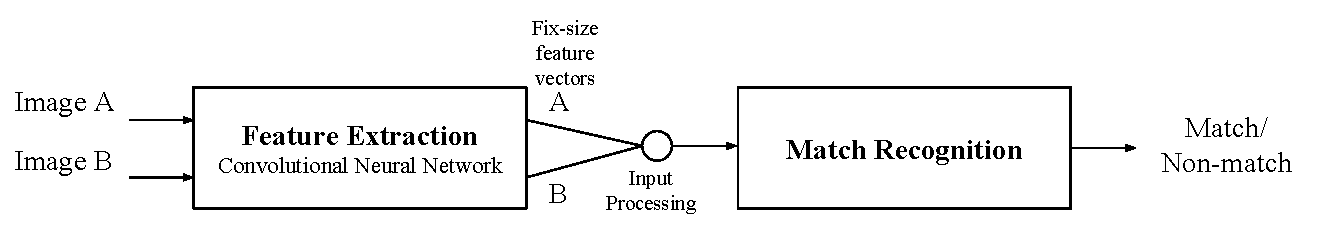
\includegraphics[width=\textwidth]{system/overview}
  \caption{System Overview}
  \label{fig:overview}
\end{figure}

\begin{enumerate}
  \item \textbf{Feature Extraction}. We use a pre-trained CNN with the last
  fully-connected layer, the output layer, removed to extract fix-size feature
  vectors from the input images before feeding them into the \emph{Match Recognition} module.
  \item \textbf{Match Recognition.}
\end{enumerate}

\subsection{Feature Extraction} 

For the pattern retrieving engine such as Sloop, the system continually
accumulates more data over time. The availability of abundant data enables the
learning based methods to thrive over the engineered features because they can
discover and optimize features for the specific task at hand.

Instead of hand-picking the features to learn the similarity matrices from the
data, a convolutional neural network (CNN) will be used as a feature extractor
similar to the solution proposed in \cite{chopra05} for face verification.

We use a pre-trained CNN, AlexNet by Krizhevsky et al. \cite{kriz12} trained on
ImageNet \cite{imagenet}, which contains 1.2 million images with 1000
categories. To convert the CNN into a feature extractor, we strip out the last
fully-connected layer, which, in this case, outputs 1000 class scores for
ImageNet classification task. According to AlexNet architecture, this would
output a sparse 4096 dimentional vector for every images. The technique is
called transfer learning \cite{transfer}.

We map all the available images as well as the input image to points in a low
dimensional space (4096-D compare to $227 \times 227$-D) using the
aforementioned CNN architecture. 

\begin{figure}[h!]
  \centering
  \subfloat[][The first layer filters, \texttt{conv1}]
    {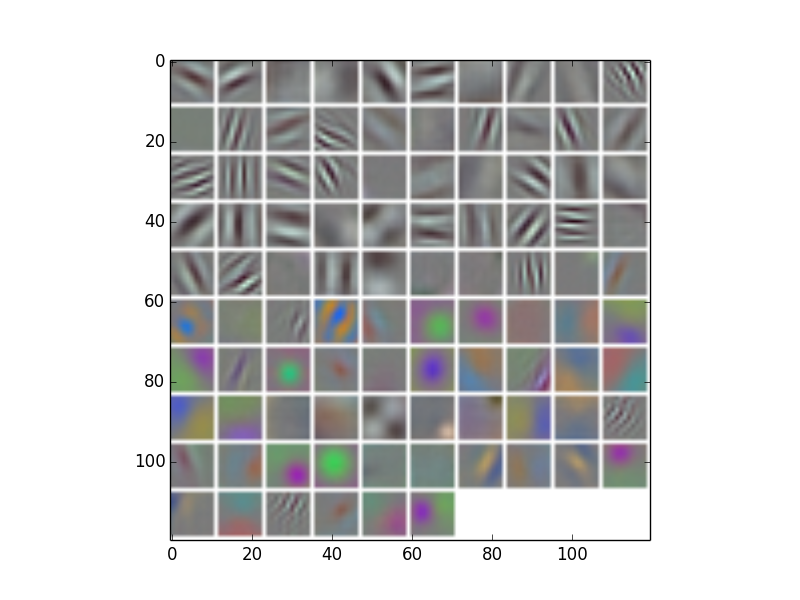
\includegraphics[width=8cm]{preprocess/paramconv1}}\\
  \subfloat[][The first layer output, \texttt{conv1}]
    {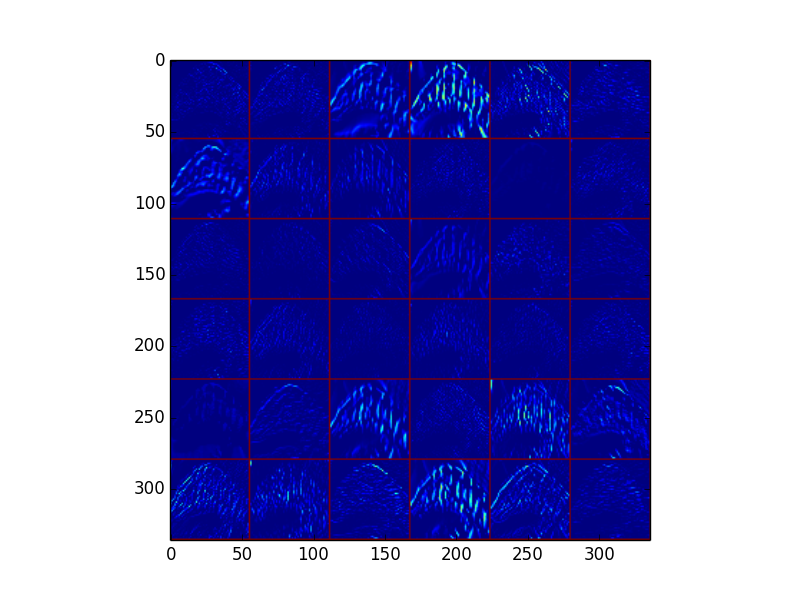
\includegraphics[width=8cm]{preprocess/blob20conv1}}
  \subfloat[][The fifth layer after pooling, \texttt{pool5}]
    {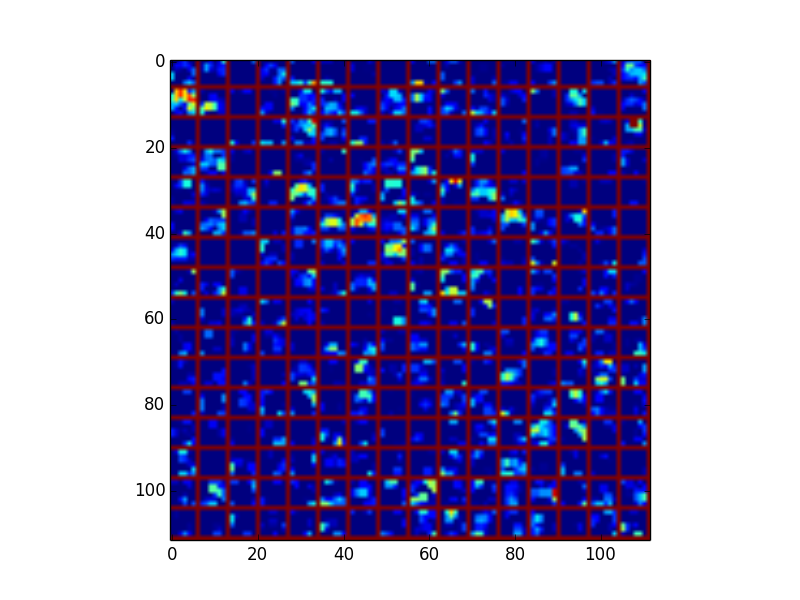
\includegraphics[width=8cm]{preprocess/blob20pool5}}] \\
  \subfloat[][The first layer output, \texttt{conv1}]
    {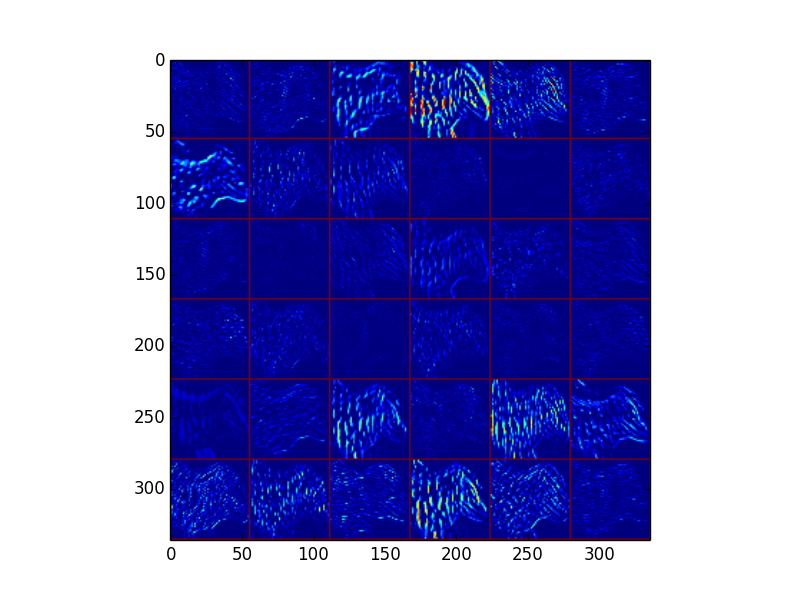
\includegraphics[width=8cm]{preprocess/lastconv1}}
  \subfloat[][The fifth layer after pooling, \texttt{pool5}]
    {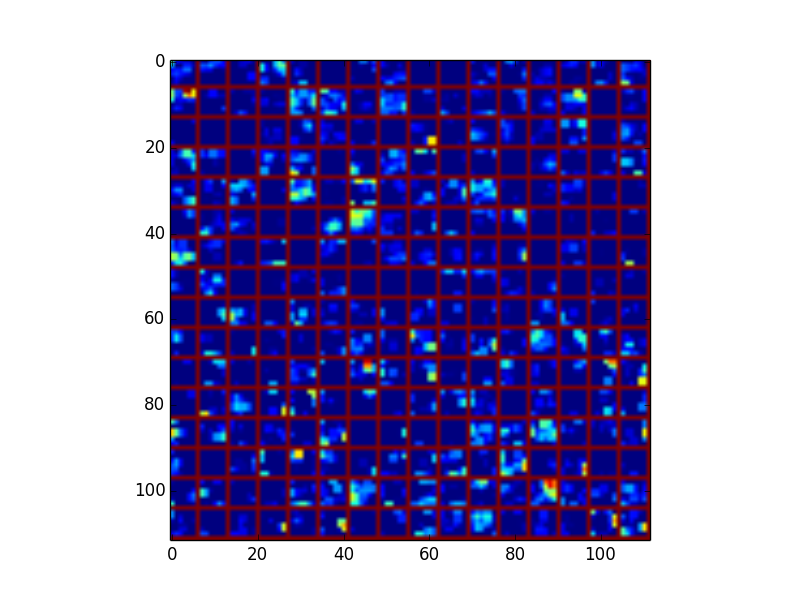
\includegraphics[width=8cm]{preprocess/lastpool5}}
  \captionsetup{justification=centering}
  \caption{Visualizing Convolutional Network layers}
\end{figure}


\textbf{Pretained Convolutional Neural Network}

The main advantage of using a pre-trained CNN to our application is that it is
robust to geometric distortion. This is a desirable property since the position
of the individuals in our dataset are not aligned. This enables us to
accurately recognize the animal regardless of its position in the image. 

The translation invariant property emerges as a result of the contiguity in our
pooling regions and the fact that we only pool features generated from the same
hidden units \cite{ufldl}. Even though the property is desirable to reduce the
translation noise, this disallows learning some features that are described by
their relative positions. For example, individual A with a star-shaped spot
right above its eye may be confused with another individual B who also has
star-shaped spot underneath its eye. 

The solution to such problem is to experiment with different pattern of pooling
regions, and relax the parameter sharing scheme. Since we are using an existing
pretrained architecture, it is hard to tailor to fit our data. The improvement
can be included in the future work \ref{future}.

\textbf{Caffe}

The CNN is implemented in python using Caffe\cite{caffe}, a deep learning
framework developed by the Berkeley Vision and Learning Center (BVLC).

\subsection{Match Recognition}

Once we have the 4096-D vectors for all images generated from our CNN feature
extractor, we transfer them into a second target match recognizer and train it
on a target dataset and task. The match recognizer is a linear classifier that,
given a pair of image vectors, decides whether the two images contains the same
individual.

\textbf{Input Processing}

Upon receiving the input from the feature extractor, we process the input using
one of the two method before passing it into the recognizer which outputs a
binary label determining whether (A, B) is a match.

\begin{enumerate}
\item Concatenation

Given two input image vectors $\vec{A}$ and $\vec{B}$ (flattened), we
concatenate them horizontally so that the output $\vec{E}$ becomes $$\vec{E} =
[ \vec{A}\, \vec{B} ].$$ To make the order deterministic, we always start with
the vector with smaller sum; otherwise, if equal sum, we compare each pair of
corresponding entries in both vectors until we find an entry with a smaller
element.

We can visualize this as feeding a tuple of image vectors $( \vec{A}, \vec{B}
)$ to a linear classifier. This is equivalent to giving the classifier all the
information we have and expect it to figure out the optimal parameters.
However, in this case there is no separator indicating that two image vectors
are actually separated.

\item Computing the absolute difference

We would like to find a similarity metric that represents how much two images
differ from each other. In order to achieve that we come up with following
metric:
$$\vec{E} = |\vec{A} - \vec{B}|$$
Each entries $e_i \in \vec{E}$ is
small if $\vec{A}$ and $\vec{B}$ belong to the same category, and large if
different.  Not only this encapsulates the desired numerical behavior, but it
also eliminates the absence of separator problem.
  
\end{enumerate}

\textbf{Recognizer}

Images can be uploaded to Sloop one by one or in a batch. One major difference
is that the batch processing keeps the system weights constant while computing
the error associated with each sample in the input, whereas the on-line version
constantly updates its weights. For the real-time system like Sloop, we would
prefer the on-line version of the classification algorithm given the same
classification performance.

We have implemented following algorithms as our match recognizer:
\begin{itemize}
  \item Linear support vector machine (SVM) with L2 regularization (squared
    Euclidean norm)
  \item SVM with radial basis function kernel (SVM-RBF), L2 regularization
  \item Perceptron (P)
  \item Passive-Aggressive with hinge loss (PA-I)
  \item Passive-Aggressive with squared hinge loss (PA-II)
\end{itemize}

We compare the performance of each classifier in the Experiments section
(\ref{experiments}). The classifier with the best performance will be selected
for our final design.

\section{Experiments} \label{experiments}

In this section, we first introduce the datasets used in the experiments, then
present the detailed evaluation of the variants of our architecture and the
comparison between the presented solutions.

\subsection{Dataset}

The training and testing data is available in the existing Sloop system. We
base our experiments on both species of skinks: \emph{Grand} and \emph{Otago}
mentioned in \ref{chap:dataset}.

For our experiments, each image from both databases is reduced to the size of
$227 \times 227$ pixels so that it can be directly fed into the CNN
architecture to speed up the feature extraction. Regardless of our preprocess,
the CNN will resize the images into $227 \times 227$ to fit its input
dimension. However, resizing is not necessary because practically our system
should maintain its identification capability without regard to the variations
in sizes, lighting, or background.

\textbf{Partitioning}

We divide the data from both databases into four datasets by animal species:
Gr$^{L}$-I, Gr$^{L}$-II, Ot$^{L}$-I, Ot$^{L}$-II where Gr is Grand, Ot is
Otago, $L$ is left view. Notice that the right view is not be used for the
experiments because the results should be similar to that of left view by
symmetry. In addition, due to our memory limit during the processing, each
dataset contains only 300 images of individuals whose image per individuals are
greater than 11.

For the purpose of generating a test set that resembles the empirical input and
another test set with images that are not seen before during training, we build
our datasets using two different techniques.
\begin{itemize}
  \item Gr$^{L}$-I, Ot$^{L}$-I represents the empirical input where the data in
  the test set can also be seen in the training set.
  \item Gr$^{L}$-II, Ot$^{L}$-II represents the test set with images that are
  not seen before during training. The set of individuals is split into three
  disjoint sets for training, validating, and testing. Each images in a set can
  only be paired with the images within the same set.
\end{itemize}

For each dataset, we partition the set of the \emph{generated pairs} into three
sets: train set (60\%), validation set (20\%), and test set (20\%)respectively.
We prevent overfitting problem by monitoring the model’s performance on a
validation set, acting as a representative of future test examples. If the
model’s performance ceases to improve sufficiently on the validation set then
we test the model on teh actual test set.


\begin{table}[t]
\captionsetup{justification=centering}
  \caption{Details of the train, validation, and test set for the four datasets}
\centering
  \begin{tabular}{lllll}
    \toprule
    \multicolumn{2}{c}{Name (NTotal)}      & NPairs & \% Match & \% Non-match \\
    \midrule
    \multirow{3}{*}{Gr$^{L}$-I (10878)}  & Train & 6526 & 0.07 & 0.93 \\
\cmidrule{2-5}
                                 & Val   & 2175 & 0.07 & 0.93 \\
\cmidrule{2-5}
                          & Test  & 2177 & 0.07 & 0.93 \\
\hline
\multirow{3}{*}{Ot$^{L}$-I (10878)}  & Train & 6526 & 0.06 & 0.94 \\
\cmidrule{2-5}
                                 & Val   & 2175 & 0.06 & 0.94 \\
\cmidrule{2-5}
                                 & Test  & 2177 & 0.06 & 0.94 \\
\hline
  \multirow{3}{*}{Gr$^{L}$-II} & Train & 2926 & 0.13 & 0.87\\
\cmidrule{2-5}
                                 & Val   & 351 & 0.38 & 0.62\\
\cmidrule{2-5}
                                 & Test  & 1035 & 0.25 & 0.75\\
    \hline
    \multirow{3}{*}{Ot$^{L}$-II} & Train & 3240 & 0.10 & 0.90\\
\cmidrule{2-5}
                                 & Val   & 561 & 0.31 & 0.69\\
\cmidrule{2-5}
                                 & Test  & 561& 0.26 & 0.73\\
    \bottomrule
  \end{tabular}
\end{table}
